Eine Spektrallampe erzeugt Licht welches anschließend gebündelt wird und durch eine Spaltblende fällt. Hinter der Spaltblende wird das Licht abermals gebündelt und durch einen Geradsichtprisma geleitet. Der Prisma teilt das einfallende Licht in seine Spektrallinien auf. Mit einer schwenkbaren Photozelle kann fast monochromatisches Licht vermessen werden. Dieser Aufbau ist in der Abbildung \ref{fig:500-3} zu sehen.
\begin{figure}[h!]
  \centering
  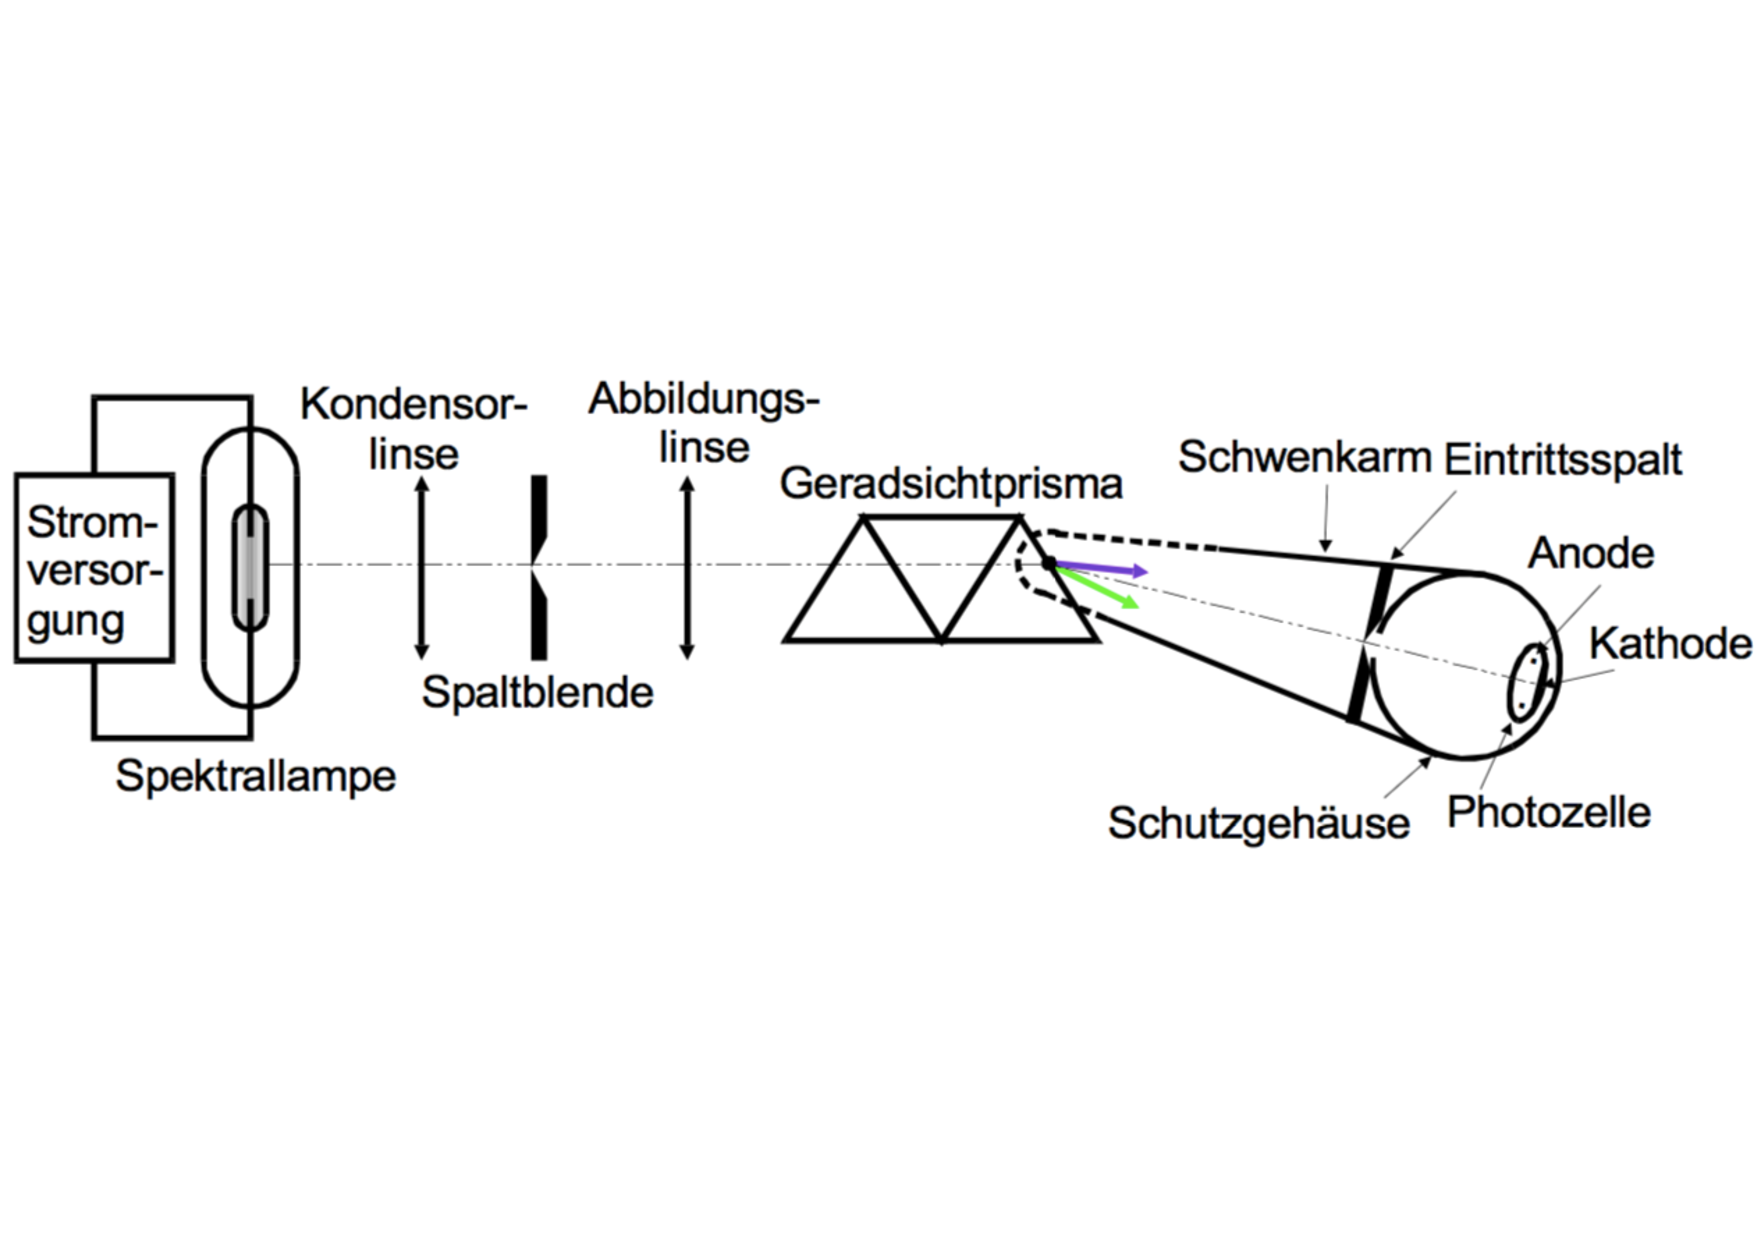
\includegraphics[width=0.8\textwidth]{500-3.pdf}
  \caption{Aufbau des Versuches \cite{1}}
  \label{fig:500-3}
\end{figure}
\\Die Photozelle ist in einem evakuierten Glaskolben, um Wechselwirkungen der Elektronen mit der Luft zu verhindern. Dieser besteht aus einer Photokathode, aus der nach Auftreffen von Photonen Elektronen ausgelöst werden können, und einer Auffängerelektrode welche für die Vermessung der Elektronen von Bedeutung ist. In Abbildung \ref{fig:500-1} ist der Aufbau der Photozelle schematisch dargestellt.
\begin{figure}[h!]
  \centering
  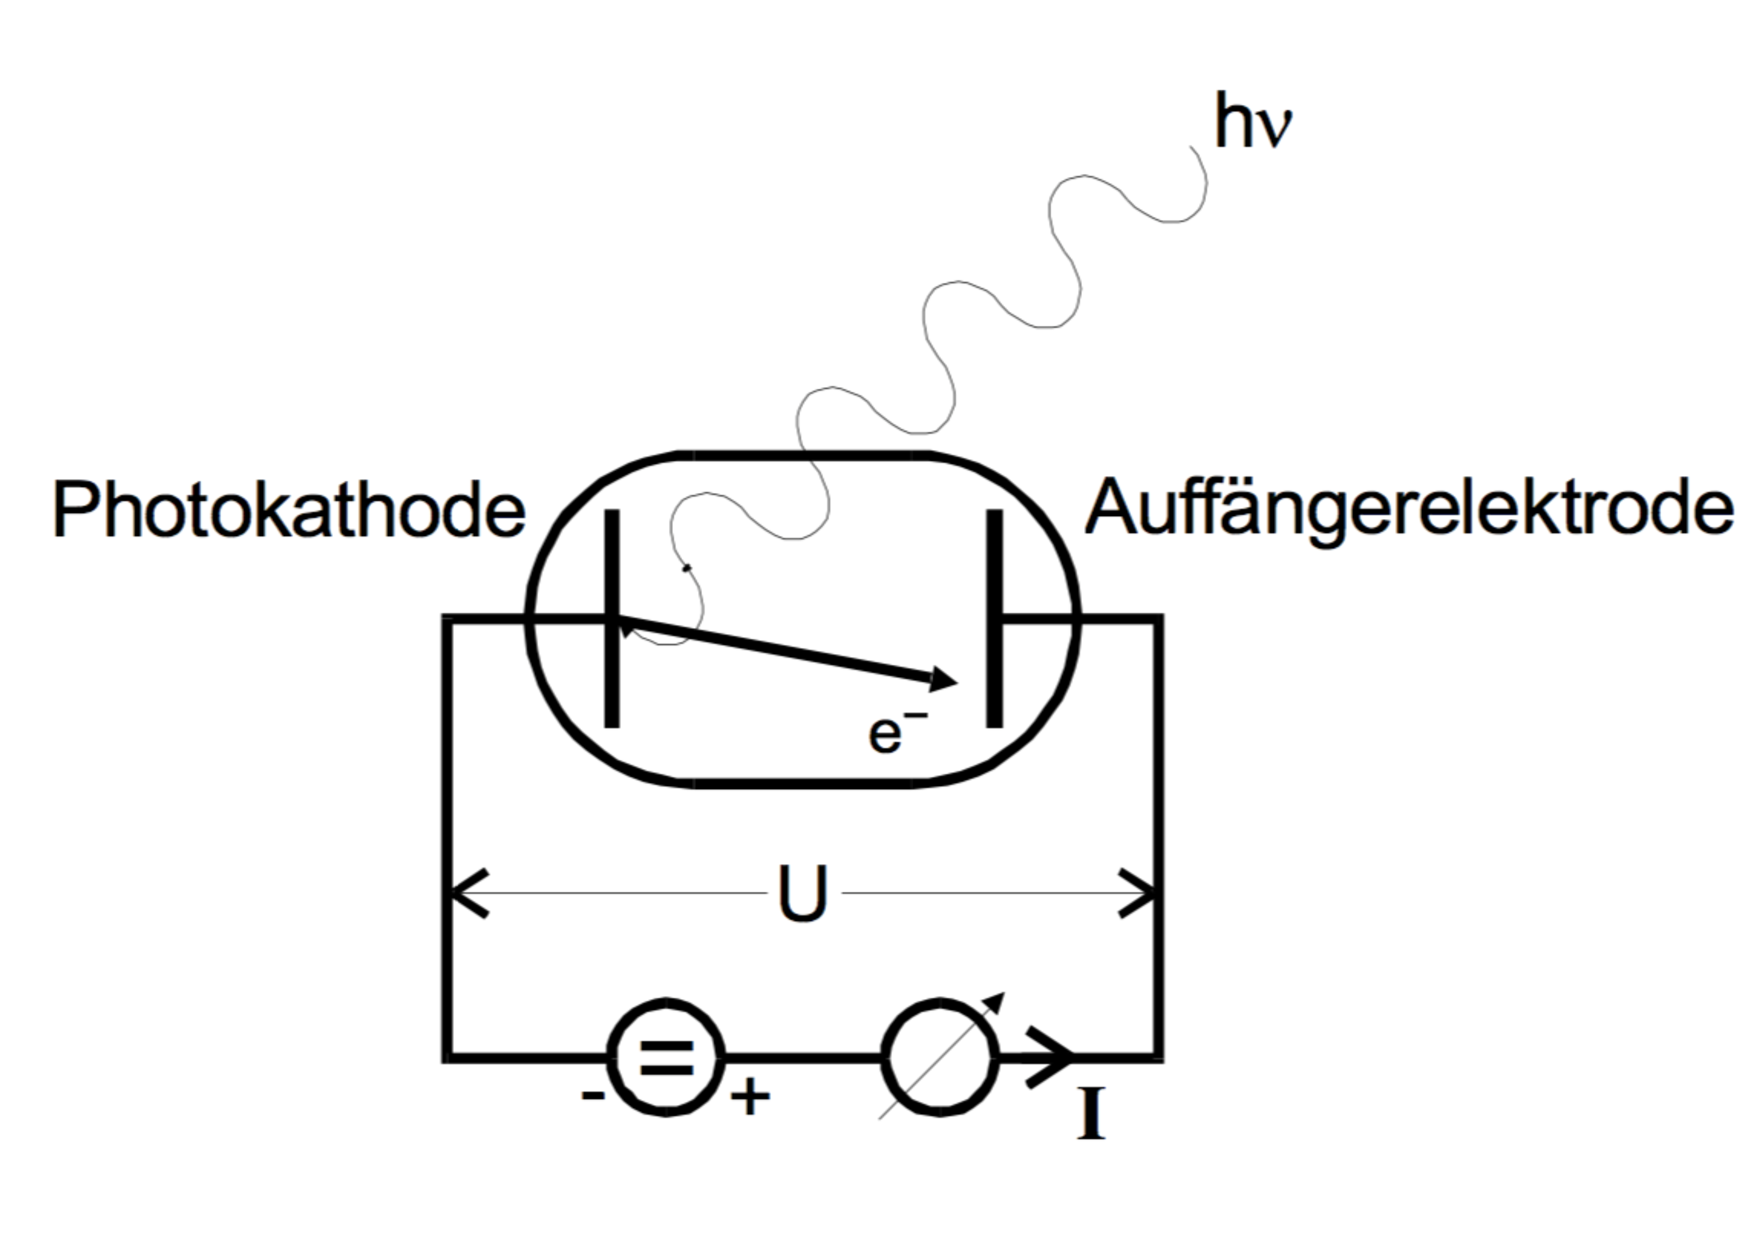
\includegraphics[width=0.8\textwidth]{500-1.pdf}
  \caption{Aufbau der Photozelle \cite{1}}
  \label{fig:500-1}
\end{figure}
\\Die Elektrode, welche mit einem Drahtring nahe der Kathode realisiert ist, misst den Stromfluss, der durch die auftreffenden Elektronen entsteht. Zusätzlich kann die Elektrode ein beschleunigendes oder abbremsendes Elektrisches-Feld erzeugen. Mit dem Elektrischen-Feld kann bestimmt werden welche kinetische Energie die Elektronen besitzen. Solange die Energie der Elektronen größer ist als die Bremsspannung $e_0U_g$ erreichen die Elektronen die Anode. Zwischen Photostrom $I_{\text{Ph}}$ und der Bremsspannung U herscht ein parabolischer Zusammenhang.
\begin{equation*}
  I_{\text{Ph}}\textasciitilde U^2
\label{eqn:e0ug}
\end{equation*}
 Der Zusammenhang zwischen dem Photostrom I und der Bremsspannung ist in der Abbildung \ref{fig:500-5} aufgetragen.
\begin{figure}[h!]
  \centering
  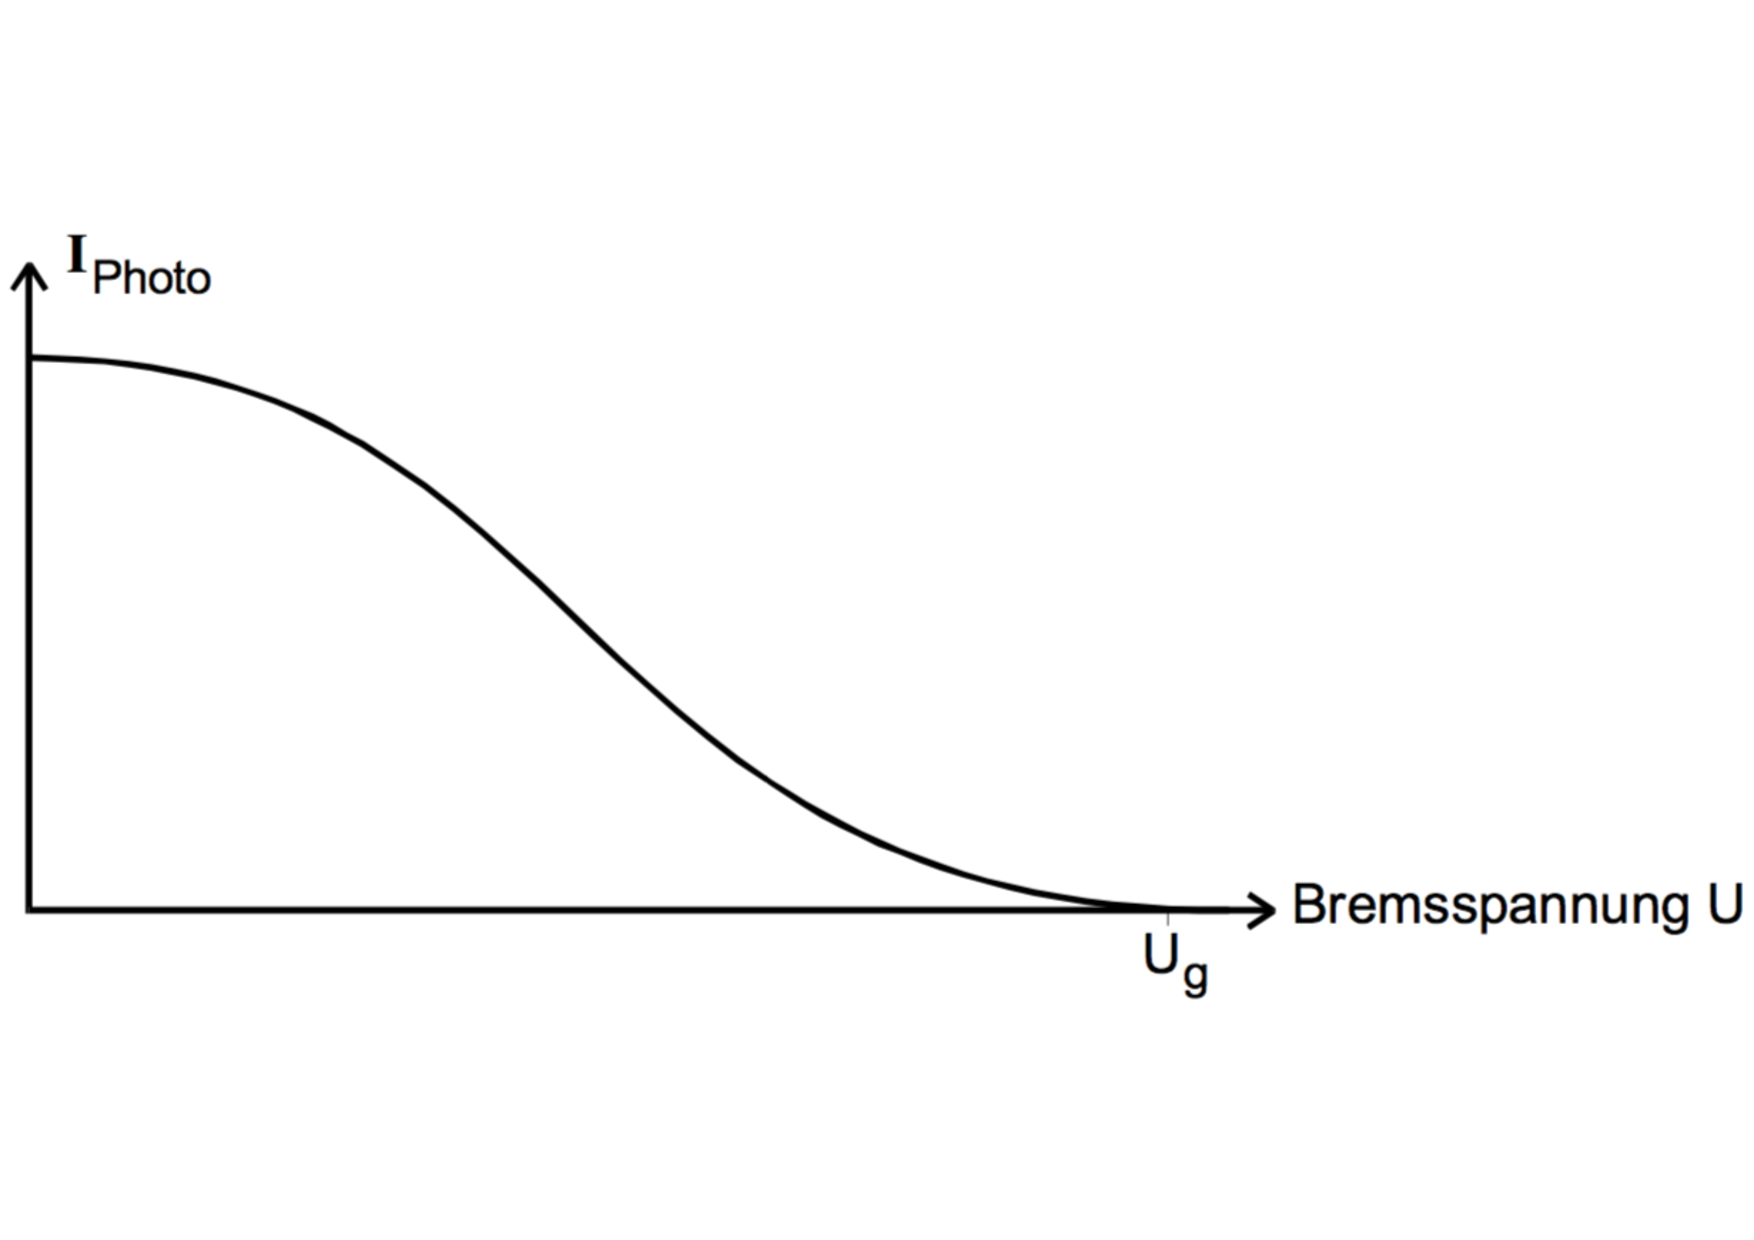
\includegraphics[width=0.8\textwidth]{500-5.pdf}
  \caption{Photostrom in Abhängigkeit von der Bremsspannung \cite{1}}
  \label{fig:500-5}
\end{figure}
\\Es kommen keine Elektronen mehr an, wenn gilt:
\begin{equation}
  e_0U_g=\frac{1}{2}m_0V^2_{\text{max}}.
\label{eqn:e0ug}
\end{equation}
$e_0$ ist dabei die Elementarladung und $m_0$ die Masse eines Elektrons. $v_{\text{max}}$ ist die Geschwindigkeit der schnellsten Elektronen.
Nach Gleichung \ref{eqn:energieE} gilt für die diese demnach:
\begin{equation}
  h\nu= e_0U_g-A_k
\label{eqn:schnellE}
\end{equation}
